
% JuliaCon proceedings template
\documentclass{juliacon}
\setcounter{page}{1}

\usepackage{amsmath}
\graphicspath{{FIGs/}}


\begin{document}

% **************GENERATED FILE, DO NOT EDIT**************

\title{DMRGenie: Graphical interface for entanglement renormalization}

\author[1]{Kiana Gallagher}
\author[1]{Aaron Dayton}
\author[2]{Drew Leske}
\author[2]{Sarah Huber}
\author[134]{Thomas E. Baker}
\affil[1]{Department of Physics \& Astronomy, University of Victoria, Victoria, British Columbia V8P 5C2, Canada}
\affil[2]{Research Computing Services, University of Victoria, Victoria, British Columbia V8P 5C2, Canada}
\affil[3]{Department of Chemistry, University of Victoria, Victoria, British Columbia V8P 5C2, Canada}
\affil[4]{Centre for Advanced Materials and Related Technologies, University of Victoria, Victoria, British Columbia V8P 5C2, Canada}

\keywords{Julia, Genie, DMRjulia, TENPACK, Entanglement Renormalization, Tensor Networks, Graphical User Interface}

\hypersetup{
pdftitle = {DMRGenie: Graphical interface for entanglement renormalization},
pdfsubject = {JuliaCon 2022 Proceedings},
pdfauthor = {Kiana Gallagher, Aaron Dayton, Drew Leske, Sarah Huber, Thomas E. Baker},
pdfkeywords = {Julia, Genie, DMRjulia, TENPACK, Entanglement Renormalization, Tensor Networks, Graphical User Interface},
}



\maketitle

\begin{abstract}

We discuss implementation of a graphical user interface for tensor operations in scientific simulations related to entanglement renormalization. We call this software DMRGenie based on its heavy reliance on Genie which is a well-known software package for web applications. We also discuss the deployment of the software. Scientific simulations with tensor network-based framework of quantum algorithm methods are now possible through this tool without lengthy start-up or learning times.

\end{abstract}


\section{Introduction}

On one hand, for ideas to be implemented computationally, a need arises for easy-to-use high level languages. "On the other hand, scientific programming often requires computational resources at scale, driving optimization and performance requirements. To accomplish this second demand, a low-level language is required to control as much as possible in an implementation of an algorithm. This split between needs for different programming projects is known as the two-language problem.

The Julia programming language is a good if not great attempt to solve this two-language problem. By optimizing for loops, programs can be created in a rapid manner but still achieve performance on par with lower-level languages such as C++. 

In any scientific endeavour, the need to use numerical techniques is highly necessary. And for new advances to be made, new methods must be able to be implemented into any given language to evolve beyond the state-of-the-art. For anyone developing new algorithms, the need for a programming framework that enables as many solutions of the two-language problem as possible is necessary, making a Julia a strong contender for algorithmic development.

%For any algorithm development team, the need for custom software that displays as many solutions of the two-language problem is necessary, making Julia a strong option for use in algorithm development.

Quantum information methods have become a tantalizing path to creating new algorithms and methods. These range from quantum algorithms implemented on quantum computers \cite{nielsen2010quantum} (but since no perfect quantum computer exist, simulations with classical methods are still required) to entanglement renormalization techniques.\footnote{This class of methods is more commonly referred to as tensor networks, simply, but with the rise of machine-learning and other methods particularly in quantum chemistry that are formulated on tensor networks, a distinguishing name is required. We choose to expand the usage of the term from Ref.~\cite{vidal2007entanglement} since all methods are fundamentally optimizing over quantities relevant for quantum information ({\it i.e.}, the entanglement) and renormalization was originally introduced to describe this class of methods \cite{wilson1983renormalization,krishna1980renormalization}. The methods required to implement an algorithm in this context is different from other contexts, notably machine learning.} 

\begin{figure}
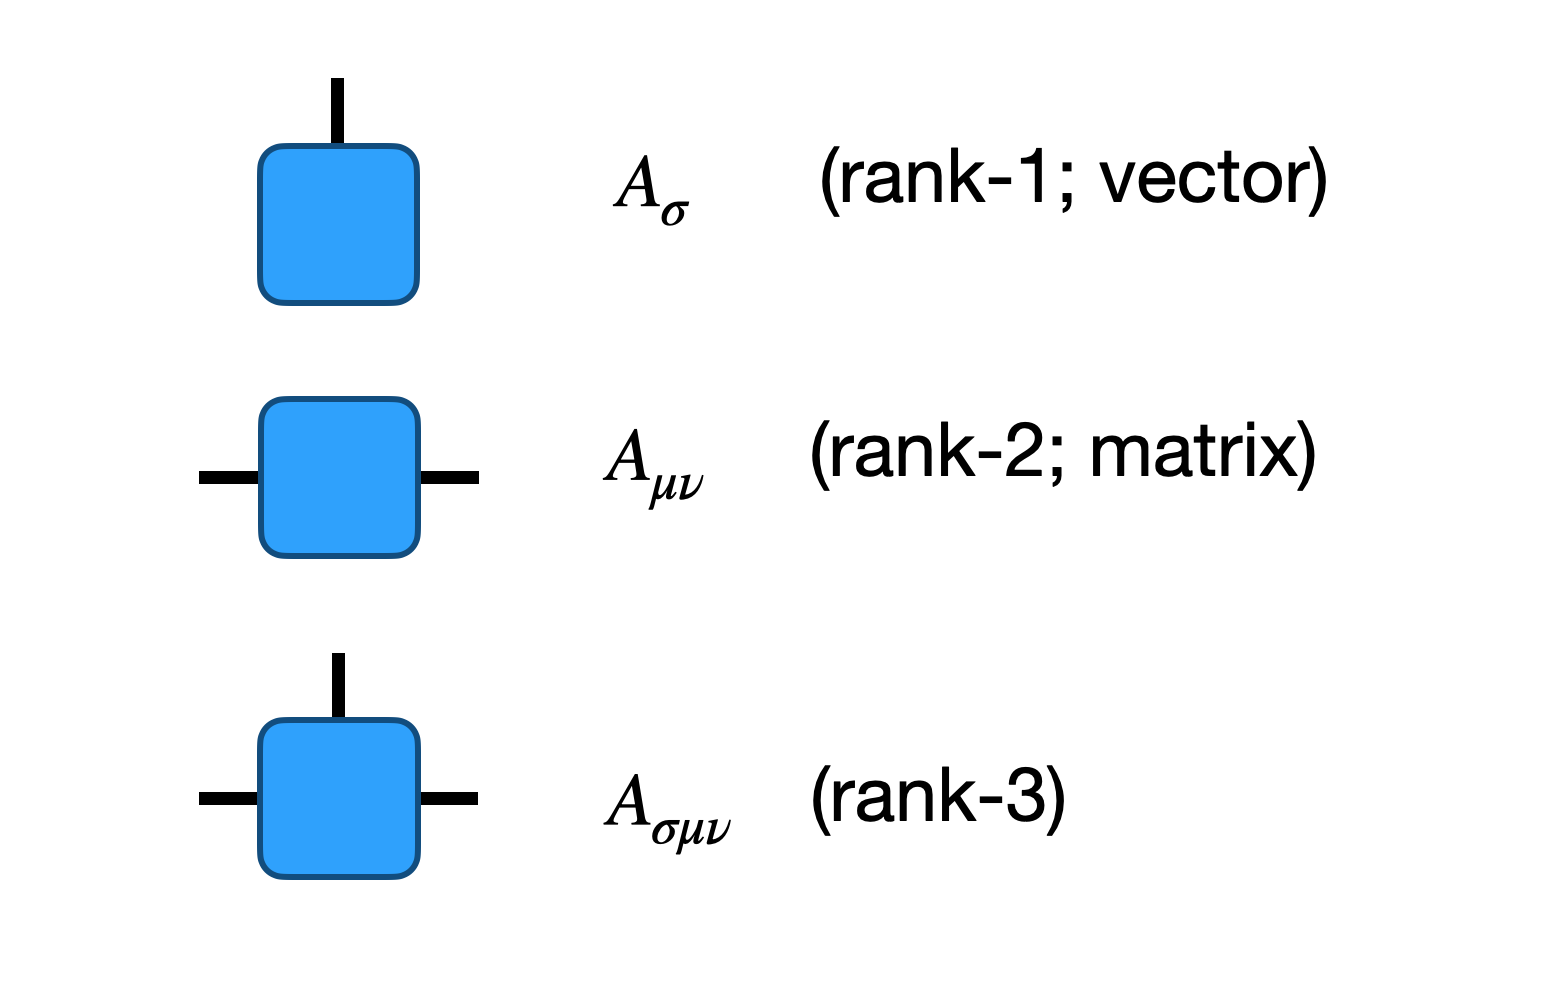
\includegraphics[width=\columnwidth]{diagram.png}
\caption{Shown are diagrams for rank-1, 2, and 3 tensors. Each line signifies another index on the tensor.
\label{diagram}
}
\end{figure}

Methods of entanglement renormalization use quantities native to quantum information ({\it i.e.}, the density matrix or the entropy) in order to optimize a a quantum problem to find solutions to the eigenvalue problem (Schr\"odinger's equation) \cite{townsend2000modern}. Entanglement renormalization techniques are formulated on a graph of tensors and have definite rules for tensor operations. Because tensor computations and operations can be cumbersome to represent mathematically in index notation, the field has adopted a diagram notation that allows for the improved communication of algorithms. Namely, the rank of the tensor corresponds to the number of lines on the diagram \cite{penrose1971angular}. An example is shown for rank-1, 2, and 3 tensors in Fig.~\ref{diagram}. 

Realistically, only about a rank-14 tensor can be represented on a laptop machine. This is because each of the tensor indices has dimension of at least two, approaching the memory limitations of these devices. Therefore, the rank of the tensors represented here are small and often only a few indices are present.

When contracting two tensors together, one can connect two indices on the same tensor ({\it i.e.}, tracing over indices) or between tensors (contraction). When representing a network of tensors, the indices are typically not kept track of. Instead, indices that point towards each other or have matching labels are assumed to be contracted eventually. This rarely causes confusion when implementing algorithms.

\begin{figure}
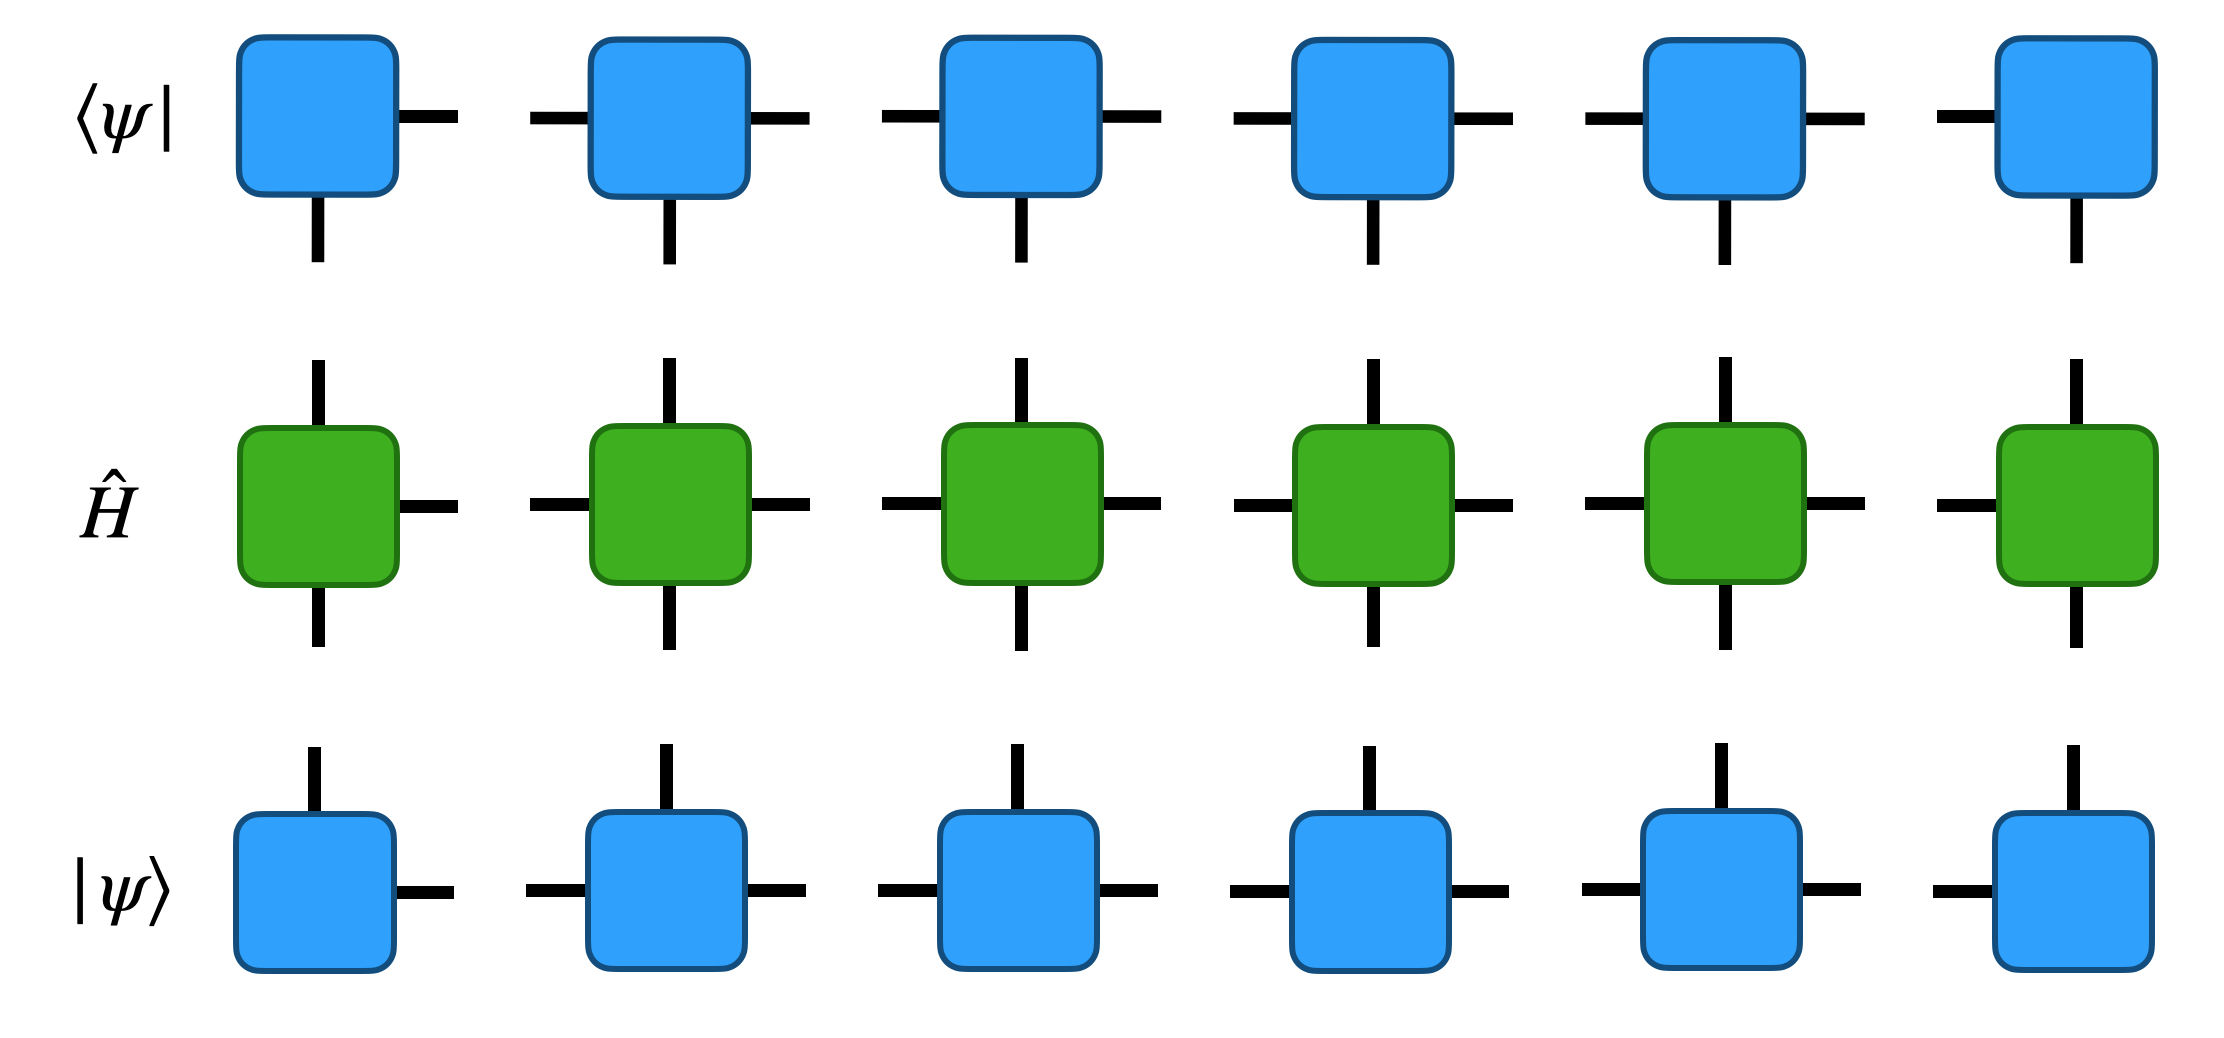
\includegraphics[width=\columnwidth]{network.png}
\caption{The expectation value of an operator $\hat H$ is shown in tensor diagram notation for a 6-site system. When contracted, this would give $\langle\hat H\rangle$, or the energy $E$ if $\hat H$ is the Hamiltonian. The wavefunction on the bottom row alone would be represented as in the text (Eq.~\ref{mpsform}), which is far more intricate.
\label{network}
}
\end{figure}

The use of the diagram notation is useful for representing large numbers of tensors in a coherent way without representing cumbersome mathematics (see Fig.~\ref{network}). For example, the wavefunction when decomposed through a series of reshapes and singular value decompositions (SVD) takes the form \cite{bakerCJP21}
\begin{align}\nonumber
|\psi\rangle&=\sum_{\substack{\sigma_1\sigma_2\sigma_3\\\sigma_4\sigma_5\sigma_6}}\sum_{\substack{a_1a_2a_3\\a_4a_5}}A^{\sigma_1}_{a_1}A^{\sigma_2}_{a_1a_2}A^{\sigma_3}_{a_2a_3}A^{\sigma_4}_{a_3a_4}A^{\sigma_5}_{a_4a_5}A^{\sigma_6}_{a_5}\\
&\quad\quad\quad\quad\quad\quad\quad\quad\times|\sigma_1\sigma_2\sigma_3\sigma_4\sigma_5\sigma_6\rangle
\label{mpsform}
\end{align}
which is far more intricate than the diagram notation but conveys no extra information. Any quantum operator (for example, the Hamiltonian) can be decomposed into a similar site-by-site form involving many tensors.

Building these algorithms from a purely diagrammatic level is a desirable possibility. This opens the possibility to using a graphical user interface to denote the various steps in the implementation of the entanglement renormalization algorithms

Julia's solution of the two-level problem allows for an easy implementation of algorithms and simultaneous fast execution of scientific code. We discuss in this article efforts to construct a fully working scientific software package for entanglement renormalization that is simultaneously fast and lightweight. This software package has then been extended to include a user interface that allows for the graphical construction of algorithms without any coding background, our principle goal here.

We will first discuss the background software (DMRjulia and TENPACK; available in Julia's package system as {\tt DMRJtensor} and {\tt TensorPACK}) originally developed in 2016 and first introduced to Github in 2020 and full debut on the Julia package environment in 2021. This means that the library has spanned many version of the Julia version starting originally in v0.5 and now continuing to v1.11 and beyond. We believe that some choices from our implementation may be interesting to the broader community, although many of the improvements that were introduced here later appeared in this development independently appeared in Julia from other groups, showing that common issues are being encountered and handled in similar ways.

DMRGenie is the natural extension of the previously developed software which we debut here. This builds on top of DMRjulia to include a graphical interface for easy development of new algorithms. This is made publicly available through a web interface and available for use with some limitations on the maximum size of the tensors and enforce reasonable computational requirements \cite{dmrgenie}.



\section{Entanglement renormalization with DMRjulia}

DMRjulia is a software package in the Julia package environment that is 100\% written in the Julia programming language. This makes the software fast and light-weight, ultimately taking only a few kilobytes to install, and optimized to the point of being as fast as lower-level implementations of the same algorithms.

The library implements several classes of tensor network anstaz to represent wavefunctions of quantum problems. This includes the matrix product state (MPS) \cite{verstraete2006matrix,baker2024bundled}, projected entangled pair states (PEPS) \cite{verstraete2004renormalization}, multiscale entanglement renormalization anstaz (MERA) \cite{vidal2007entanglement}, and classical tensor network algorithms such as the tensor renormalization group (TRG) \cite{levin2007tensor}. Each of these implementations is done with care towards ease of use, culminating in the DMRGenie implementation here.  All of these tensor networks are implemented in a fully flexible way.

The algorithms can be accessed and coded in a variety of styles from the basic manipulation of tensors with four basic operations (reshaping, permuting tensors, contraction, decomposition) \cite{bakerCJP21,baker2019m,dmrjulia1}. Other operations such as joining tensor indices together (as a generalization of the direct sum operation on vectors or matrices) is also available. 

We have also introduced a {\tt nametens} system to attach strings to each tensor index and formulate rules such that the {\tt *} operator is overloaded to find all common names and contract them.\footnote{Details on all functions in the library are available by typing {\tt ?} followed by the name of the function in the Julia terminal.} This provides another interface to develop algorithms that is useful in some cases.

The implementation here for methods of entanglement renormalization is given as 100\% of Julia code with no dependencies beyond the basic library.\footnote{As of this article, the library is in an extended beta-testing phase. As we add more users, we are creating useful error checks for algorithms that can be created. The library will be moved to the alpha phase after this is complete, and we welcome feedback and development from anyone even if this phase has passed.}

\section{Tensor algebra with TENPACK}

The issue of type stability has been of paramount concern to ensure that any code developed in the language avoids generating too much overhead because of Julia's multiple dispatch capabilities. Since the compiler in Julia must assume that any possible input can be entered into a function, the assumptions of how types are converted and exactly what type is created can generate excess allocations which ultimately slow a program. Eliminating these excess allocations is necessary to create efficient code that is competitive with lower level languages.

For example, when reshaping a tensor, the rank of the tensor changes. The implementation of the basic {\tt Array} type in Julia contains both the element data type and also the rank of the tensor. Because the rank of the tensor is a fluid quantity in entanglement renormalization methods, this naturally creates issues with the base implementation of Julia's library and a desire to reduce allocations for greater efficiency with an alternative struct.

As a bridge between the operations on tensors in DMRjulia and Julia, as well as the lower level BLAS functions that Julia relies on, the Tensor (Linear Algebra) Package (TENPACK) was created. The package is implemented entirely in Julia with no dependencies beyond the basic Julia implementation.

The basic tensor type in TENPACK is the {\tt denstens} abstract type which has the {\tt tens} struct. This closely mirrors the definition of the {\tt Array} type in base Julia, but it only records the element type of the tensor. There are two fields for this struct: {\tt .size} (to store the current size of the tensor) and {\tt .T} field (storing the elements of the tensor as a vector, no matter the current shape). The {\tt .size} field contains a {\tt Memory} type that was recently introduced in v1.11. This means practically that this implementation will allow for better determination of the type when using these custom structs and throw allocations in some non-standard places ({\it i.e.}, when the size field is requested as a tuple, the {\tt Memory} in {\tt .size} is converted to a tuple generating one allocation). We find overall that the changes we imposed make for a faster implementation especially on smaller systems, although it is difficult to compare fully because it is merely a trade-off and makes compilation into an executable easier, particularly with the recently developed trimming feature to make executables far smaller than previous implementations.

The design choices of TENPACK purposefully backtracks somewhat on the original promise of Julia in that most every function is fully typed for fixed inputs, so the code is not fully flexible and makes a stronger play for efficiency over flexibility. This can make the lowest levels of the library somewhat more difficult to maintain and manage with future feature improvements. However, we are able to run scalable simulations in this library that is created entirely in Julia.

We also found it necessary to re-code some of the basic Julia functions into a form that natively admits the {\tt tens} type. Notably, the implementation of {\tt permutedims}, {\tt setindex}, and {\tt getindex} were coded to avoid issues when updating versions that sometimes caused type instabilities, although care is taken to ensure that these functions (and others such as {\tt svd}) are as efficient as the base Julia library). %avoid the use of the {\tt Cartesian} coordinates features. While these improvements are definitely a slick and universal implementation, we noticed that in some versions of Julia's release that there were some type stabilities generated by converting the {\tt tens} type to an {\tt Array} and then using the base Julia features. We therefore coded a more traditional implementation of these functions and noticed that the number of allocations throw is less by an order of magnitude for {\tt permutedims} and {\tt getindex}. For most permutes requested, {\tt permutedims} is also faster. We find {\tt getindex} is faster in almost every case. By making custom functions, this is also stable between versions of Julia.
The goal when doing in this in the library is to always to match the performance and memory consumption of the basic Julia functions, but we want to ensure type-stability across versions. In some cases, a more rudimentary version of the function is used \cite{press1992numerical} or an alternative LAPACK function is called to ensure stability on the types of input tensors we provide.\footnote{For example, the basic implementation of {\tt svd} now uses {\tt LAPACK.gesdd!} (divide and conquer method) but this can return an error in some cases that we have noticed for our inputs. The {\tt svd} function in TENPACK natively calls {\tt LAPACK.gesvd!}. For the faster divide and conquer method, we have made a new function {\tt fsvd} (fast SVD, divide and conquer) and similar to still provide access to this and we do use this in some cases.}



The original hope for Julia was to solve the two-language problem, and that is still largely solved in DMRjulia and TENPACK. We have merely made some compromises to ensure that there is efficient implementation because our use case is narrower than the most broad implementation that Julia strives to deploy.

%but some of these developments are not forwarding that goal at least for our purposes. We do not question the implementation in standard Julia functions as this kind of drift towards more specific functions and rewriting some basic functions was bound to happen for a more specific use case. We merely point out that some of these features are different for this library.


\section{Graphical interface with DMRGenie}
The DMRGenie graphical user interface (GUI) allows for tensor network algorithms to be run with minimal to no coding required, and using diagrams which are easier to read. DMRGenie consists of the Algorithm Runner and the Tensor Network Builder. The Algorithm Runner executes tensor network algorithms such as the density matrix renormalization group (DMRG) using known models or custom Hamiltonians \cite{dmrjulia1}. The Tensor Network Builder allows the user to build their own tensor network and create their own tensor network algorithm using a drag-and-drop system. The frontend was built using HTML, JavaScript, React, and CSS for styling. The backend uses a Model View Controller (MVC) infrastructure. The packages used to run the tensor network algorithms are DMRjulia and TENPACK. So, while both DMRjulia and TENPACK are 100\% from-scratch Julia implementations, DMRGenie is not, but this makes the code easier to use and work with and adapt to changing software standards in the future.

\subsection{DMRGenie Backend}\label{backend}
The DMRGenie website was built using a Model View Controller (MVC) infrastructure, which was initialized using the Genie.jl Julia package. Genie was chosen because it allowed for full-stack development with Julia as the backend. This improved the development cycle as it made it simple to run tensor network functions with DMRjulia and TENPACK. The models and controls are written in Julia, while the views are written in Julia and HTML using a \texttt{.jl.html} file extension with supporting JavaScript files for functionality. 

The model is a struct which is used to pass data between the frontend and backend of the application. 
When a page is initially loaded, a model is initialized with a default set of data. Once the user inputs their options and submits, that raw data is sent to the backend where tensor network computations can then be performed accordingly.

The view file contains the HTML for the application. This file is capable of containing Julia code due to its ".jl.html" file extension, allowing the controller to pass Julia variables to be output on the frontend. 

The controller is responsible for starting up the HTML page with the relevant data when the website is initialized. When a tensor network is created or a tensor network function is run, the controller is responsible for creating the tensors and running the algorithm using DMRjulia and TENPACK. The results of any operation are stored in variables and returned to the view component.

Much of the data collection is handled in the routes. When a computation is submitted, the routes receives this request, parses through the data, then sends it in a usable format to the corresponding controller. Data is sent to the backend in a POST request and collected using the \texttt{postpayload} Genie function for the Algorithm Runner, while for the Tensor Network Builder it is sent as JSON then parsed using the JSON3 Julia package.

\subsection{DMRGenie Frontend}
The two main components of DMRGenie are the tensor network builder and the algorithm runner. The frontend of DMRGenie was built using HTML, CSS, and JavaScript along with ReactJS. The only ReactJS component of the app was the Tensor Network Builder. ReactJS was used along with ReactFlow which is a package meant for building node-based editors and interactive diagrams. 

\subsection{Algorithm Runner}
The Algorithm Runner is an interface that allows the user to build their own models or run known models to get the ground state energy of the system. The number of sites for a system and its Hamiltonian must be specified. The current supplied Hamiltonians are for the Hubbard model, the $t-J$ model, and the Heisenberg model \cite{fradkin2013field}. Custom Hamiltonians can be built by the user by specifying the physical dimension of the system, the Hamiltonian constant, and the components of the Hamiltonian.


\begin{figure}
\begin{center}
    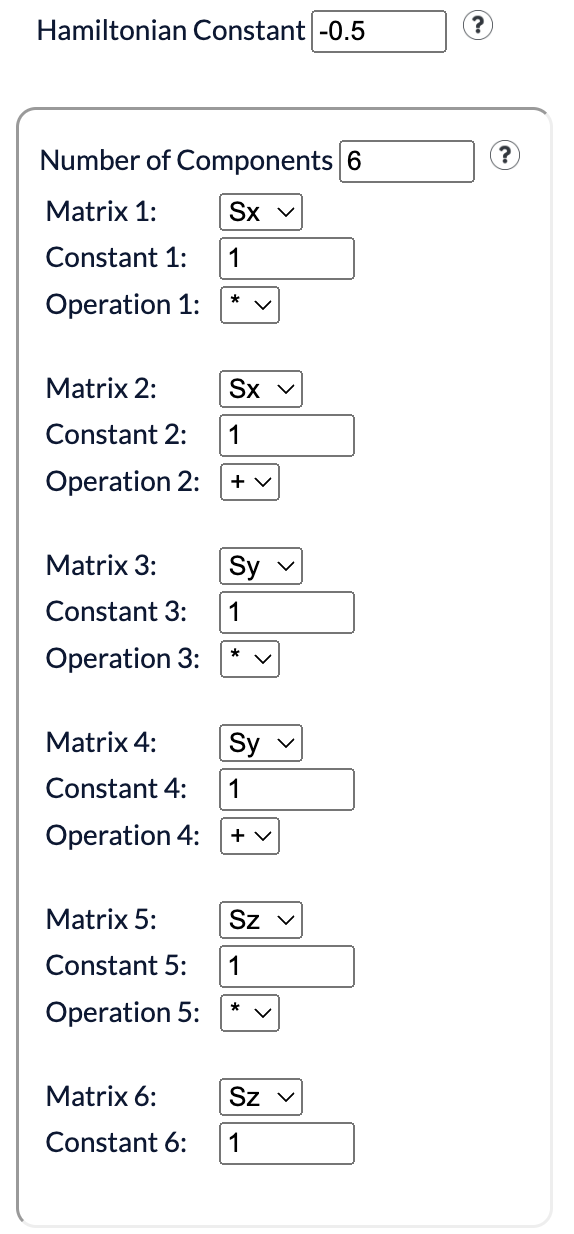
\includegraphics[scale=0.5]{HeisenbergModel.png}
\end{center}
    \caption{The Heisenberg Model input for the Algorithm Runner written term-by-term as in Eq.~\eqref{heisMPO}.
    \label{heismodel}
    }
\end{figure}

For example, if the user wanted to input a Heisenberg Hamiltonian of 
\begin{equation}\label{heisMPO}
\hat H = -J\sum_{i} \left( \sigma^x_i \sigma^x_{i+1} + \sigma^y_i \sigma^y_{i+1} + \sigma^z_i \sigma^z_{i+1}\right)
\end{equation}
where $J$ is the Hamiltonian constant, then it would be possible to do so term by term. An example of the input is given in Fig.~\ref{heismodel}.

It is also possible to compute the correlations and impose symmetries on the system. The correlation matrix operators and correlation function operators must be specified to compute correlations. The matrix operators and function operators will then be evaluated at all positions on the lattice. 

Details of the symmetries and how they need to be implemented are included in Appendix~\ref{qsymmetries}.




\subsection{Tensor Network Builder}

The Tensor Network Builder is a drag and drop interface to build tensor networks. The rank of any tensor is specified before they are dropped onto the canvas. The number of connections points on a tensor is equal to the rank of the tensor. Indices can be created by dragging from a connection point on a tensor. It is possible to specify the name and dimension of all indices, and it is possible to rename an index if needed. Possible operations on tensors include contractions (see example of interface in Fig.~\ref{GUIcontraction}), singular value decompositions, eigenvalue decompositions, QR decompositions, and LQ decompositions. When the user is done, the "submit" button can be clicked and the algorithm will be run on the backend. The output of the algorithm will be the tensors that resulted from the last operation. The output is given as a downloadable file.

ReactJS is used for the tensor network builder because of component reusability and the fast rendering. The ReactFlow package was designed to build node-based editors and interactive diagrams; however, graphs in computer science have similar structures to tensor networks. The nodes and edges in ReactFlow were generalized to tensors and indices. 


\begin{figure}
    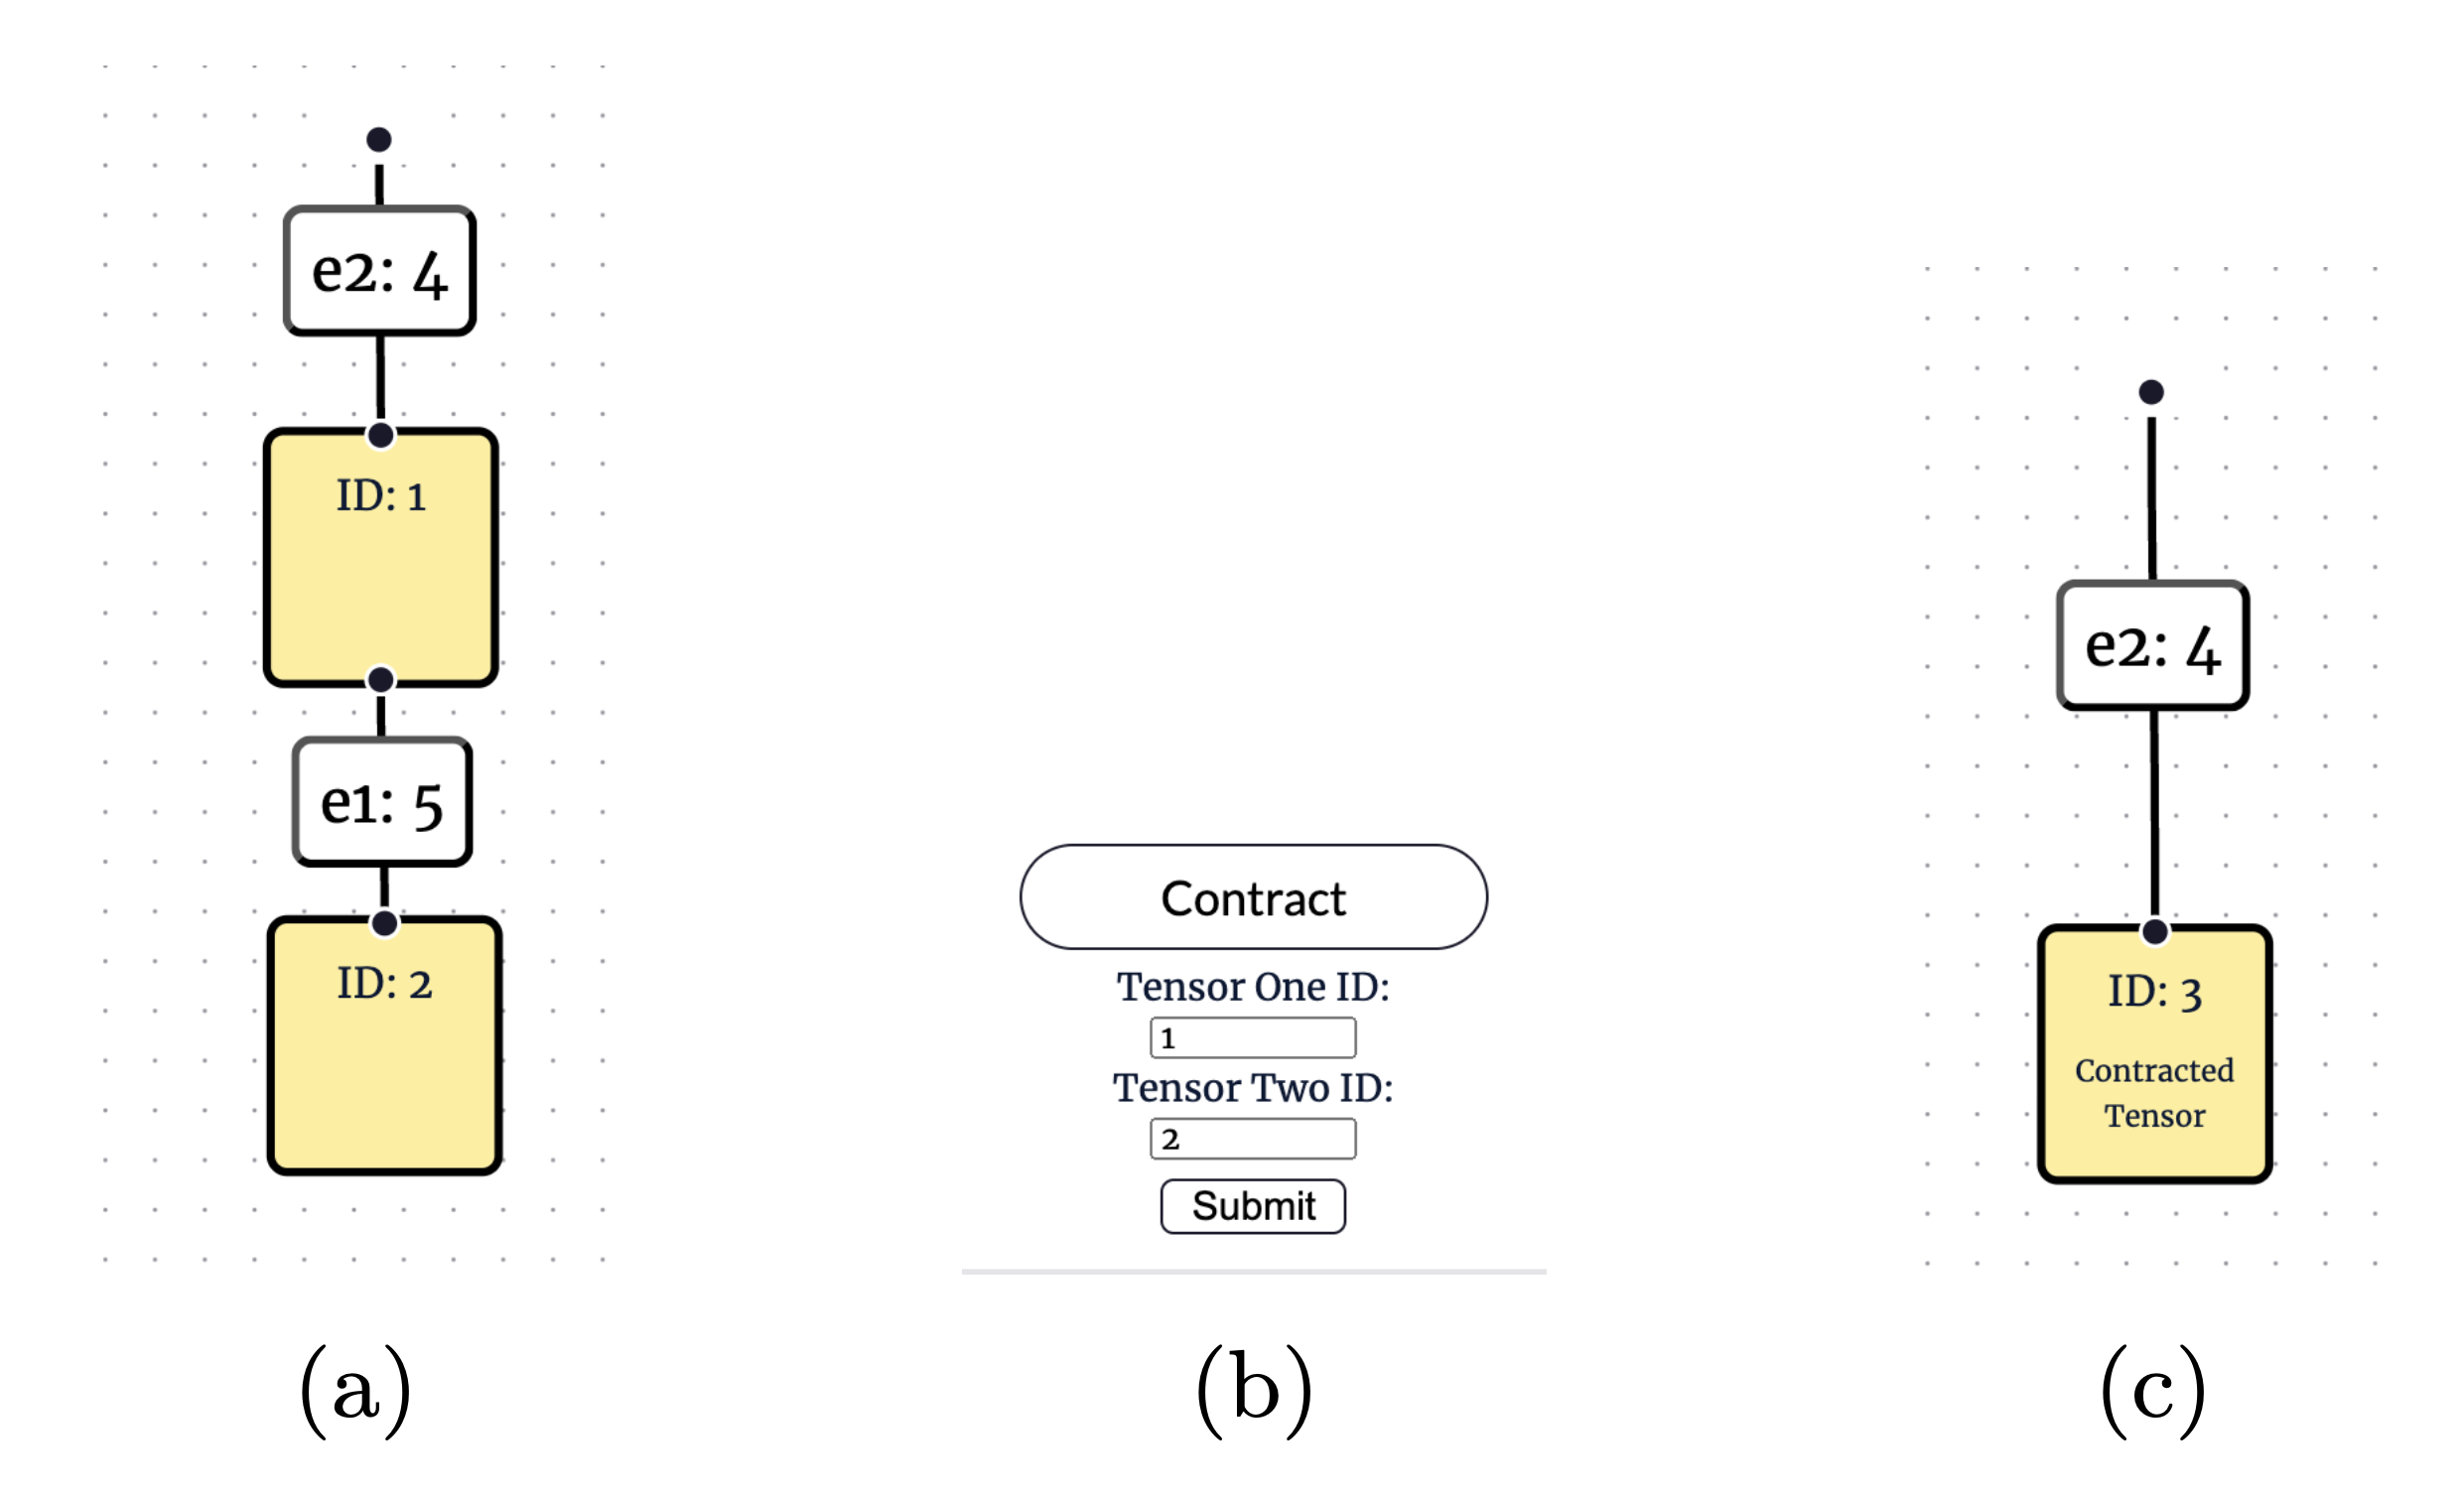
\includegraphics[width=\columnwidth]{contraction.png}
\caption{Contraction two tensors with the Tensor Network Builder interface. a) The initial tensors. b) The input given to the contract menu operation. c) The output tensor. } \label{GUIcontraction}
\end{figure}

\section{Deployment}
%-uses resources supplied by the Research Computing services at the Unviersity of Victoria\\

The application is packaged into a Docker container using GenieDeployDocker and Docker tools.  The container image is then pushed to a local image registry and scanned for vulnerabilities before deployment to a Kubernetes cluster, where it is made available on the web.  The registry,  cluster and web access are components of a self-serve application deployment platform.

\section{Conclusion}

A graphical user interface for entanglement renormalization has been presented here in DMRGenie. This builds upon the previous DMRjulia and TENPACK packages to make coding novel quantum algorithms far easier and more visual. 

\section{Installation and usage}

The basic libraries for DMRjulia and TENPACK can be obtained from online repositories \cite{dmrjulia,tenpack} or from the Julia package environment:
\begin{lstlisting}[language = Julia]
julia> ]
pkg> add DMRGenie DMRJtensor TensorPACK
\end{lstlisting}

The DMRGenie GUI can be used online \cite{dmrgenie}.

\section{Acknowledgement}

K.G.~acknowledges support from the Valerie Kuehne Undergraduate Research Award, the Undergraduate Student Research Award (USRA) from NSERC, and the Summer Emerging Undergraduate Award (SERA) from the Faculty of Science at the University of Victoria. 

K.G.~and A.D.~acknowledge the NSERC CREATE in Quantum Computing Program, grant number 543245.

A.D.~acknowledges the Jamie Cassel's Undergraduate Research Award (JCURA). A.D.~acknowledges support from the Undergraduate Student Research Award (USRA) from NSERC.

This research was undertaken, in part, thanks to funding from the Canada Research Chairs Program. The Chair position in the area of Quantum Computing for Modelling of Molecules and Materials is hosted by the Departments of Physics \& Astronomy and of Chemistry at the University of Victoria. 

This work has been supported in part by the Natural Sciences and Engineering Research Council of Canada (NSERC) under grants RGPIN-2023-05510 and DGECR-2023-00026, and ALL-RP 590857-23.

This research was enabled in part by support and resources provided by the Research Support Services at the University of Victoria.

This work was supported by the Digital Research Alliance of Canada.


% **************GENERATED FILE, DO NOT EDIT**************

\bibliographystyle{juliacon}
\bibliography{ref.bib}


\begin{appendix}


\section{Running locally}

DMRGenie can be run locally and we show how to do this here.

\subsection{Setup}

Navigate to the `tensez` directory once the repository has been cloned and then into the `TensEZ` folder within it.

Install the necessary packages with instantiate.

\begin{lstlisting}[language = Julia]
julia> ] 
pkg> instantiate
\end{lstlisting}

\subsection{Running the App}

The app must be activated by running the following from the `TensEZ` directory

\begin{lstlisting}[language = Julia]
julia> ] 
pkg> activate .

julia> using Genie
julia> Genie.loadapp()
\end{lstlisting}

\section{Quantum symmetries}
\label{qsymmetries}

TENPACK currently supports local $U(1)$ and $\mathbb{Z}_n$ symmetries. The basic idea is to establish the relevant quantum numbers on each physical index (drawn as the vertical index on the MPS). Specifying the quantum numbers on each of the physical indices is sufficient to determine the quantum numbers on all other indices, provided that the total flux of the input Hamiltonian is a net zero ({\it i.e.}, symmetry-preserving Hamiltonian). Given this case, all tensors exhibit a block structure, where each block has a set of non-zero values and no non-zero values are available between quantum number sectors.

Given a symmetry preserving Hamiltonian, one can use rules similar to Kirchoff's loop rules (with total flux equal to zero) to determine the quantum numbers on each index. All of this is automatically handled in the quantum number tensor implementation in TENPACK for abelian quantum numbers. 

For example, consider the Hamiltonian for two spin-half objects on two different sites
\begin{equation}
\mathbf{S}_1\cdot\mathbf{S}_2=\frac14\left(\begin{array}{cccc}
1 & 0 & 0 & 0\\
0 & -1 & 2 & 0\\
0 & 2 & -1 & 0\\
0 & 0 & 0 & 1\\
\end{array}\right)
\end{equation}
where $\mathbf{S}=\boldsymbol{\sigma}/2$ for the Pauli vector $\boldsymbol{\sigma}$ \cite{townsend2000modern} and subscripts denote which site the spin vector is located. The matrix can be divided into three blocks, and in general, we can write a block structure of completely independent pieces as
\begin{equation}
\mathbf{S}_1\cdot\mathbf{S}_2=1\oplus\left(\begin{array}{cc}
-1 & 2 \\
2 & -1
\end{array}\right)\oplus1
\end{equation}
where $\oplus$ is a direct sum. Each of these three independent pieces can be assigned a quantum number (+1, 0, -1; in order). This means that if we were to multiply this matrix with another matrix respecting the same symmetries, we could break the full matrix multiplication into parts. In this case, consider multiplying $\mathbf{S}_1\cdot\mathbf{S}_2$ by itself and noting that one could perform three matrix multiplications, one on each quantum number sector, and obtain the same result.

This idea generalizes to all tensors that respect a quantum number symmetry. When reshaping an index, one can simply sum the abelian quantum numbers together to find the quantum number on the resulting grouped index. Eventually, one will need to contract a tensor. By identifying which indices are contracted and which are not, one can reshape any tensor into a matrix that must be divisible into quantum number blocks.

The implementation in TENPACK has been optimized so that it is fast. This methodology also avoids any issue with numerical round-off error accidentally changing the desired quantum number sector for a given problem. For example, not imposing quantum number symmetries for fermions can lead to a loss or gaining a fermion, which may resulting in finding an answer for a different symmetry sector than was originally intended. it is recommended to use quantum number symmetries whenever the problem displays quantum numbers.


\section{Builder's guide}
The frontend for the Tensor Network Builder was built using HTML, CSS, JavaScript, and React. It is recommended that the developer has experience in these languages. The majority of the interface is coded in React, and the styling is done in CSS. The React package used is \textbf{ReactFlow}. This specific package was chosen because it is used to create graphs commonly found in computer science, and the package was well documented. Computer science graphs and tensor networks have quite a bit of overlap in their structure. The nodes and edges can easily be generalized to tensors and indices. The website has two main components: the network canvas and the drag and drop menu.

Any functions called using ReactFlow are of the form \textbf{ReactFlow.FunctionName()}. This was due to an issue importing ReactFlow into the Genie environment. It should be noted that all the ReactFlow elements should be inside the $<$\textbf{ReactFlow.ReactFlowProvider}$>$ element as this is the ReactFlow environment. 

\subsection{Network Canvas}

The network canvas is where the tensor network is displayed. The current canvas is provided by the ReactFlow package. The network canvas is a \textbf{div} element inside the $<$\textbf{ReactFlow.ReactFlowProvider}$>$ element. The canvas is where the tensors are displayed, moved, and edited.

The $<$\textbf{ReactFlow.ReactFlow}$>$ element is used to specify the functions called when specific events occur. These events include deleting tensors, deleting indices, moving tensors, and validating connections. If no function is passed through the element then the default functions are used which can be found on the ReactFlow website documentation. The $<$\textbf{ReactFlow.Controls}$>$ element is for the controls at the bottom left corner of the canvas. The $<$\textbf{ReactFlow.MiniMap}$>$ element is for the mini version of the canvas at the bottom right. The $<$\textbf{ReactFlow.Background}$>$ element is for the background of the canvas


\subsection{Drag and Drop Menu}
The drag and drop menu allows the user to create random tensors, upload tensors, and apply operations on created tensors. It is contained inside the $<$\textbf{ReactFlow.ReactFlowProvider}$>$ element. The drag and drop menu has a tag of $<$\textbf{DNDMenu}$>$. It also contains all the elements for the tensor operations.

The variables that are used for all the tensor operations are passed through the drag and drop menu element. The drag and drop menu also keeps track of which operation is currently active and only allows one active operation at a time. This was a design choice, but it is not necessary.

\subsection{Tensors}
Nodes in ReactFlow are created by making an object in JavaScript that has specific properties and passing it to the \textbf{setNodes} function. This function will create a node on the canvas with the specified values. The object must contain certain properties such as \textbf{id}, \textbf{position}, and \textbf{type}. There are properties that are optional such as \textbf{style} and \textbf{data}. There is no strict limit to the properties, but any custom properties should be passed through the value linked to the data property.

Two custom nodes were created to represent tensor networks. The two types are \textbf{tensor} and \textbf{invisible}. The code for these tensors can be found in \textbf{TensorNode.js} and \textbf{InvisisbleNode.js}. To make the simplest node, a empty div element can be returned, but we want to be able to connect tensors. The $<$\textbf{ReactFlow.Handle}$>$ element is used to create a handle that allows edges to be connected to it. So a custom node is created by creating a div and specifying the handles and any other desired HTML or React elements .The tensor type is used to represent a tensor in a tensor network. The invisible type is required for free indices because the package required edges to have two connection points.

When creating a tensor type node, the \textbf{data} value is an object that must include certain properties such as the \textbf{rank} as an Int, \textbf{mutable} as a boolean, \textbf{label} as a string, and \textbf{color} in the form of an Int from 1-100. Furthermore, the style property is an object that should include a \textbf{backgroundColor} property in the form of a string; it is currently "hsl(" + tensorColor + ", 100\%, 80\%)". If the tensor is being created by uploading then the data property must also include a \textbf{input} property as a string. The string is currently "", but this can be changed. 

In the case of an invisible node, it is much simpler. The \textbf{data} value must contain a \textbf{mutable} property which should be a boolean value. 

The rank of the tensor is equal to the number of handles for the tensor, so a tensor of rank 3 can have only have 3 connection (a connection to any type of node is considered a connection). Additionally, the IDs must be unique, so a \textbf{nodeId} variable is incremented every time a tensor node is created. Similarly, if an invisible node is created then its ID is `f\$\{freeNodesId\}` where \textbf{freeNodesId} is incremented every time an invisible node is created. If a node is deleted then all its edges will be deleted or split. If the tensor is connected to another tensor then that edge will be split otherwise the edge will be deleted.This is done by the \textbf{onNodesDelete} event.

\subsection{Indices}
Connecting two tensors is done by dragging from one handle of a tensor to a handle of another tensor. Free indices are created by dragging from a handle of a tensor onto the network canvas.
Similar to nodes, edges are created by making an object in JavaScript with specific properties and passing it to the \textbf{setEdges} function. This function will create the edges on the canvas. The object must contain certain properties such as \textbf{id}, \textbf{sourceX}, \textbf{sourceY}, \textbf{targetX}, \textbf{targetY}, \textbf{sourcePosition}, \textbf{targetPosition} and \textbf{type}. There are properties that are optional such as \textbf{style} and \textbf{data}.

Similar to the nodes, custom edges can be made. There is only one type of custom edge required which is of type \textbf{index}. The code for the edge type can be found in \textbf{DimensionEdge.js}. For an index type edge, the data value must contain the property \textbf{dim} which is a positive Int, \textbf{chosenDim} which is a boolean, and \textbf{lineStyle} which is "Bezier" or "Free". The dimension of an index is immutable, so once the user choses the index then \textbf{chosenDim} becomes true. The \textbf{lineStyle} is "Free" if the edge is connected to an invisible type node otherwise it is "Bezier".

Since IDs must be unique, if a edge is created then it's ID is `e\$\{eId\}` where \textbf{eId} is incremented every time an invisible edge is created. If an edge is deleted and it connected to an invisible node then the invisible node will be deleted as well. This is done by the \textbf{onEdgesDelete} function.


\subsection{Contract}
The contract operation accepts two different tensor IDs and contracts the tensors with these IDs. The contraction will cause the two tensors to be replaced with a new tensor that represents the contraction of the original tensors. The two tensors are contracted along indices that are named the same. Therefore an index that directly connects two tensors will be contracted. 
If tensor one and tensor two both have an index labeled the same thing and they are the same dimension then that index will also be contracted along. This is done by deleting the given two tensors and all indices that are being contracted along. Any indices that are not contracted will still be connected to the new resulting tensor.

An error will occur if the contraction is invalid or too many indices have the same name, or either tensor does not exist.

\subsection{SVD Decomposition}
The SVD composition accepts the ID of a single tensors and two groups of the tensor's indices. The decomposition will result in 3 tensors. The tensors will be two complex unitary matrices and a diagonal matrix. This is done by replacing the original tensor by these 3 tensors. The tensor that results from the first group of indices will be connected to the tensors that the original edges were connected to (excluding the original tensor) and the diagonal matrix. The same applied to the tensor produced by the second group of indices. Th diagonal matrix is connected to the unitary matrices.

Errors will occur if the matrix does not exist or not all the indices are grouped properly.


\subsection{QR/LQ Decompositions}
The QR/LQ decomposition accept the same input as the SVD decomposition. The resulting tensors will be the Q(L) and R(Q) matrices if the QR(LQ) decomposition is done.  The tensor that results from the first group of indices will be connected to the tensors that the original edges were connected to (excluding the original tensor). The same applied to the tensor produced by the second group of indices.

An error will appear if the original tensor does not exist or the indices are not grouped properly.


\subsection{Eigenvalue Decomposition}
The eigenvalue decomposition accepts the ID of a single tensor are returns three square matrices. These matrices are the diagonal matrix of eigenvalues, the matrix of eigenvectors, and the matrix of inverse eigenvectors. This is done by replacing the original matrix with these square matrices and connecting them (in the order of eigenvectors-eigenvalues-inverse eigenvectors). 

An error will occur if the selected tensor is not isolated or it is not a square matrix.

\subsection{Split Edge}
Splitting an edge does not change the tensors in the backend, but it makes the tensor network easier to understand visually. Splitting an edge takes the label of the edge as input. The tensors that the original edge is connected to will then be connected to an invisible tensor instead.

This is done by creating two new edges and two new invisible nodes. The new edges will have the same label as the original edge.

\subsection{Connect Edge}
Connecting an edge does not change the tensors in the backend, but it makes the tensor network easier to understand visually. Connecting edges accepts two edge labels that are connected to invisible nodes as input. It will then connect the tensor nodes directly. This is done by deleting the two original edges and replacing it with a single edge. The new edge will have the label of the first input edge. 

An error will occur if the dimension of the indices do not match or one of the indices does not exist.

\subsection{Copy and Paste}
Tensors are copied by selecting a group of isolated tensors and either clicking the copy button or using \textbf{command+c}. It does not matter if an edge or a invisible node is selected. An error will occur if the tensors are not isolated. First, the copy function will gather all the tensors that have been selected. It will then copy all the invisible nodes connected to the tensor nodes. The edges connected to all nodes are then copied. The copying step requires the IDs of all edges, and nodes to be updated as they must be unique. Furthermore, the target/targetHandle and source/sourceHandle must be updated for all the edges or they will connect to the original target and source.

Pasting what has been copied will add the saved nodes and edges to the network canvas. In the case that the original tensor(s) need to be duplicated multiple times then the pasting function will preform a copy on the current copied contents. This guarantees that it is possible to duplicate the same thing multiple times. Otherwise the IDs would not be unique and thus would cause bugs. 


\subsection{Undo and Redo}
A history is saved for each operation. The status of each tensor and edge is saved as a history, so it possible to revert the status. If a new operation is done then the previous history will be rewritten.

\subsection{Adding New Operations}
Adding new operations requires the frontend to produce an accurate representation of the operation being done. It is easiest to use tensor IDs and edge labels as the input. Once those have been identified, it is important to determine which edges or nodes must be removed, updated, or added. It is possible to get the lists of nodes and edges using const \textbf{getNodes} and \textbf{getEdges}. It is then possible to set the nodes and edges using \textbf{setNodes} and \textbf{setEdges}. These functions can be called using \textbf{ ReactFlow.useReactFlow()}.

\subsection{Connecting to Backend}
When an operation is done, it passes the name of the operation done and the JavaScript objects of the tensors and edges involved.

\subsection{Chosen Conventions}
\begin{itemize}
	\item \textbf{invisible} nodes are \textbf{ALWAYS} the target node, never the source. Changing this will cause some errors in the code.
\end{itemize}

\subsection{Additional Info}
\begin{itemize}
	\item Multiple elements can be selected by \textbf{holding command+clicking}
	\item React elements must start with a capital letter or errors may occur (this is a convention but it is easy to forget when learning)
\end{itemize}


%Make sure that the path ends with `tensez/TensEZ`, if not then run `{\tt cd("<path\_to\_repo>/tensez/TensEZ")}` from the Julia CLI.
%
%Then exit the Pkg prompt with *backspace*.
%
%Run the following commands
%
%\begin{lstlisting}[language = Julia]
%julia> using Genie
%julia> Genie.loadapp()
%\end{lstlisting}


%
%\onecolumn
%
%\section{Developer's guide}
%
%%\section{INTRODUCTION}
%
%This document covers how to add/modify features in the DMRGenie webapp. DMRGenie is built on a Model View Controller (MVC) infrastructure. For information on the implementation of the MVC framework with basic functionality, the package decisions, or how to run the app, see the \lstinline|Readme.md| file. Some information is common between these documents.
%
%Many instructions can be found in the Genie documentation \href{https://genieframework.github.io/Genie.jl/dev}{here}. For example, to learn how to create a new MVC group read \href{https://genieframework.github.io/Genie.jl/dev/tutorials/4-1--Developing_MVC_Web_Apps.html}{this} page.
%
%\subsection{File structure}
%
%The main folder of concern for editing the application is \lstinline|DMRGenie/app/resources|. Within this folder, all the models, views, and controllers are sorted into distinct folders. As of May 16, 2024, the only group included is the \lstinline|tensornetwork| group. A supporting folder is \lstinline|DMRGenie/public|. The file \lstinline|DMRGenie/routes.jl| handles the exchange of data between the front and back end.
%
%\subsubsection{The \lstinline|tensornetwork| MVC group}
%
%Within the resources folder is the \lstinline|tensornetworks| directory, which contains \lstinline|TensorNetworks.jl|, \lstinline|TensorNetworksController.jl|, \lstinline|views|, and \lstinline|TensorNetworksValidator.jl|.
%
%The file \lstinline|TensorNetworks.jl| contains the tensor network model. Think of it as an object which can be passed between the front and back end of the application. If you want any data to be exchanged between these ends, then you must include a new field with a default value in the model. Make sure that variable names are descriptive and follow the same format as existing names. Note that modifying this file requires a full restart of the application.
%
%The file \lstinline|TensorNetworksController.jl| contains the tensor network controller. This is responsible for serving up the HTML page with the relevant data. The main function within this file is \lstinline|DMRGenie| which is run in \lstinline|DMRGenie/routes.jl| when the website is first started and when a tensor network algorithm is subsequently run.
%
%When the application is first started up \lstinline|DMRGenie()|, with no input, is run. This generates a default tensor network as defined in the model, which is then passed into the \lstinline|html| function from Genie. The \lstinline|html| function takes the MVC group name (in this case \lstinline|:tensornetworks|), the desired view name (in this case \lstinline|:DMRGenie| corresponding to the file \lstinline|views/DMRGenie.jl.html|), and any additional input fields required by the view.
%
%When a tensor network is built by the user and sent to the back end, it is processed by the \lstinline|DMRGenie/routes.jl| file, which builds the desired \lstinline|TensorNetwork| type (which just holds metadata) and sends it to \lstinline|TensorNetworksController.jl|. In \lstinline|TensorNetworksController.jl| the actual Tensor Network is produced in terms of MPS and MPO, then the desired algorithm is run on it with \lstinline|DMRJtensor|. The results are then stored in variables and passed through the \lstinline|html| function to be served up to the user.
%
%The folder \lstinline|views| contains the HTML for the application. As of May 16, 2024, the only file in this folder is \lstinline|DMRGenie.jl.html|. This file defines the landing page of the application: every box, button, option, color, and word is included here or in another file linked to it.
%
%Notice the file type of \lstinline|.jl.html|. This indicates that the file is capable of running Julia code. To do this you must enclose any Julia code in \lstinline|$(...)|. Only data passed in via the \lstinline|html| function may be accessed in this file by invoking the same name. For example, \lstinline|hamiltonain_measurement| is passed into \lstinline|html| and is accessed by \lstinline|$(hamiltonain_measurement)|, or \lstinline|tensor_network| is passed into \lstinline|html| and the \lstinline|default_model| field of it is accessed by \lstinline|$(tensor_network.default_model)|.
%
%JavaScript code can be run within an HTML file as well. External JS files and inline scripts are included at the top level within \lstinline|<head>|. For example, the line \lstinline|<script src="/js/drawing.js"></script>| makes the functions within \lstinline|DMRGenie/public/js/drawing.js|, like \lstinline|update()|, available to the HTML file. Another example of JS being used in the file would be in something like the \lstinline|onclick| field of a button which calls a JS function when a click action is performed on the button in question: \lstinline|onclick="HideOrShowCorrelationOptions()"|.
%
%Learning HTML is crucial. Google is your best friend when working with it. Many components have already been built for other applications and are readily available in articles or stack overflow posts. It is often difficult to get spacing to work nicely in HTML right away, so it is recommended that you create every piece of a new feature in an ugly way before making it look nice to avoid redoing work.
%
%The file \lstinline|TensorNetworksValidator.jl| currently has no support with our application, but this should be added. Refer to DMRGenie documentation \href{https://genieframework.github.io/Genie.jl/dev/}{through this link}.
%
%
%\subsubsection{Public}
%
%Another important folder is \lstinline|DMRGenie/public|. Within it are \lstinline|js|, which contains the JavaScript,  \lstinline|css|, which contains the styling CSS files, \lstinline|img|, which contains any images or gifs, and \lstinline|usergenerated|,  which contains any user generated data such as downloadable output files. If you make any new JavaScript files, CSS files, images, etc., then they should go in the corresponging folder.
%
%The \lstinline|usergenerated| folder is for files generated by the user. As of now, partial density matrices are saved into files and given to the user as available downloads. This is done quite sloppily and will likely need to change. When the application is booted up this directory is automatically cleared, but this could cause issues with multiple users using the application at once. The files do not need to be kept around long term so a database may be overkill. It is unclear if it is a best practice to have them just sitting in the public folder though. \textit{A decision will need to be made about this.}
%
%
%
%\subsubsection{Routes}
%
%The final important file of note is \lstinline|DMRGenie/routes.jl|, which handles all the data transfer from the front end and back end via HTTP methods, such as POST requests, and the application bootup process.
%
%There is one main POST request for the webpage currently which computes the following steps:
%
%\begin{enumerate}
%  \item Initialize all the necessary variables
%  \item Begin a try-catch block for error handling in the case of malformed data or unforseen issues
%  \item Get the data passed from the front end, stored in the name attribute of some tag, with the \lstinline|postpayload| function which takes a Symbol of the corresponding name and the default value. The \lstinline|parse| function is used in the case of numerical data.
%  \item Create a new \lstinline|TensorNetwork| and pass it to the controller via the \lstinline|DMRGenie| function.
%\end{enumerate}
%
%The most complicated part of this process is parsing the data via \lstinline|postpayload| functions, since each field must be handled individually. All it boils down to is just getting the name of what data you want to read, reading it, then storing it in the correct format. If there is some unknown number of fields which must be read, then use a loop to iterate the names with the same naming convention as is used on the front end until no data is recieved from \lstinline|postpayload|.
%
%It should be noted that the this setup is fragile in some ways. The application must be restarted if the names of any routes are changed. Sometimes a fill compute restart is required to get things working again.
%
%The \lstinline|DMRGenie/routes.jl| file also handles the startup of the application with the following lines:
%
%\begin{verbatim}
%  up()
%
%  file = open("bootup.log", "w")
%  write(file, "INITIALIZATION COMPLETE")
%  close(file)
%\end{verbatim}
%
%The \lstinline|bootup.log| file is there for the deployment infastructure to work. When a docker image is deployed using the containerized application, the startup sequence is run through Julia Genie commands and the deployment infastructure must wait until this is done. So it waits to read the \lstinline|bootup.log| file, and once it does the webpage is made available.
%
%
%\subsection{Deployment}
%
%To deploy the DMRGenie website one must build a docker image, and deploy it on dockerhub. This section covers the relevant basics of docker and how to deploy.
%
%\subsubsection{Dockerfile}
%
%There are three steps in the dockerization of an application:
%
%\begin{enumerate}
%  \item Creating a dockerfile
%  \item Turning the dockerfile into an image
%  \item Booting up the image into a container environment where code can be executed
%\end{enumerate}
%
%To deploy the application, it is turned into an image with Docker and deployed using software developed by Drew Leske of ARCsoft.
%
%See the dockerfile for how the docker image and container are built (each command is a ''layer''). The docker image is public on dockerhub due to a requirement of the deployment software by Drew Leske of ARCsoft.
%
%Any dockerfile consists of a list of ordered commands which build layers of a docker image when built. The containerized version of the application is basically a specification for a computing environment. Docker images are made from the container and function as the environment where processes can be run. So what we built for Drew Leske is an image, which his software uses to instantiate docker container instances, which are then run on computing nodes when requests are made to the website.
%
%Documentation for docker can be found \href{https://docs.docker.com/}{here}. Our dockerfile is built as follows:
%
%\begin{itemize}
%  \item Specify a base image you wish to build on top of. For example, you could build on a specified version of the Ubuntu or Alpine docker images. We use the latest version of the julia image for linux/amd64
%  \item Configure the environment: create directories, copy files over, edit permissions, etc.
%  \item Add any packages used in the application
%  \item Specify ports and environment variables
%  \item Run the application via a CMD instruction. The server file specified just contains the line which starts the application: 
%\begin{lstlisting}[language = Julia]
%julia --color=yes --depwarn=no --project=@. -q -i -- $(dirname $0)/../bootstrap.jl -s=true "$@"
%\end{lstlisting}
%\end{itemize}
%
%
%\subsubsection{How to deploy}
%
%To deploy there are a few simple steps which we will write in plain English first, then in the CLI commands to be executed. The terminal commands should be executed in the \lstinline|dmrgenie/DMRGenie| directory which holds the dockerfile. Before doing any of that though, make sure you have Docker Desktop installed.
%
%\begin{enumerate}
%  \item Build a docker image with a tag specifying the version (i.e. \lstinline|v0.2.1|)
%  Command:
%  %\lstinline|
%  
%\begin{lstlisting}[language = Julia]
%  docker build -t <Your Docker Hub Account>/dmrgenie:v0.2.1 . #(Make sure to change the version tag!)
%\end{lstlisting}  
%  
% 
%  \item Deploy the image with the same tag to dockerhub
%  Command:
% %\lstinline|
%\begin{lstlisting}[language = Julia]
% docker push <Your Docker Hub Account>/dmrgenie:v0.2.1 #(Make sure to change the version tag!) 
% \end{lstlisting}
% 
%  \item Email Drew Leske that a new docker image is up. Make sure to tell him the version tag (in this case we would tell him the new docker image is at \lstinline|<Your Docker Hub Account>/dmrgenie:v0.2.1)|!
%\end{enumerate}
%
%So far, all docker images have been deployed to aarondayton87/dmrgenie, but you will need to deploy them to your personal repo. You can see this public repo on dockerhub for a history of versions though.
%
\end{appendix}






\end{document}

% Inspired by the International Journal of Computer Applications template
